% =============================================================================
%  IconGenAI: Fine-tuning a Code LLM for Text-to-SVG Icon Generation
%  via the Iconify Corpus
% =============================================================================
%
%  Template: NeurIPS-style (adapt to target venue by swapping \documentclass)
%  Build:    pdflatex main && biber main && pdflatex main && pdflatex main
%  Overleaf: upload all files under study/ and compile main.tex
%
% =============================================================================

\documentclass[10pt, a4paper]{article}

% --- Packages ---
\usepackage[margin=1in]{geometry}
\usepackage{hyperref}
\usepackage{graphicx}
\graphicspath{{../notebooks/output/}{../output/}{figures/}}
\usepackage{booktabs}       % professional tables
\usepackage{multirow}       % multi-row cells
\usepackage{amsmath}
\usepackage{amssymb}
\usepackage{listings}       % code listings
\usepackage{xcolor}
\usepackage{float}
\usepackage{caption}
\usepackage{subcaption}     % subfigures
\usepackage{microtype}      % better justification
\usepackage[style=authoryear, backend=biber, maxnames=99, url=true, doi=true, natbib=true]{biblatex}
\usepackage{siunitx}        % \num{275912} → 275,912 with thousand separators
\addbibresource{references.bib}

% --- Brand colors ---
\definecolor{brandblue}{HTML}{006EC7}
\definecolor{brandpurple}{HTML}{461EBE}
\definecolor{brandorange}{HTML}{FF9868}
\definecolor{brandpink}{HTML}{F566BA}
\definecolor{brandteal}{HTML}{28DCAA}
\definecolor{brandgreen}{HTML}{76C800}

% --- Code listing style ---
\lstdefinestyle{svgstyle}{
    language=XML,
    basicstyle=\ttfamily\footnotesize,
    keywordstyle=\color{brandblue},
    commentstyle=\color{brandblue!50},
    stringstyle=\color{brandblue!80},
    breaklines=true,
    frame=single,
    rulecolor=\color{brandblue},
    xleftmargin=1em,
    xrightmargin=1em,
}

% --- Custom commands ---
\newcommand{\method}{IconGenAI}
\newcommand{\dataset}{Iconify-SVG}
\newcommand{\todo}[1]{\textcolor{brandorange}{\textbf{[TODO: #1]}}}

% =============================================================================
\begin{document}

\title{\method: Text-to-SVG Icon Generation via\\
       Fine-tuning of a Code Language Model}

\author{
  Yauheniya Varabyova \\
  adesso SE \\
  \texttt{yauheniya.varabyova@adesso.de}
}

\date{April 2026}
\maketitle

% --- Model comparison figure (page 1, before abstract) ----------------------
\begin{figure}[H]
  \centering
  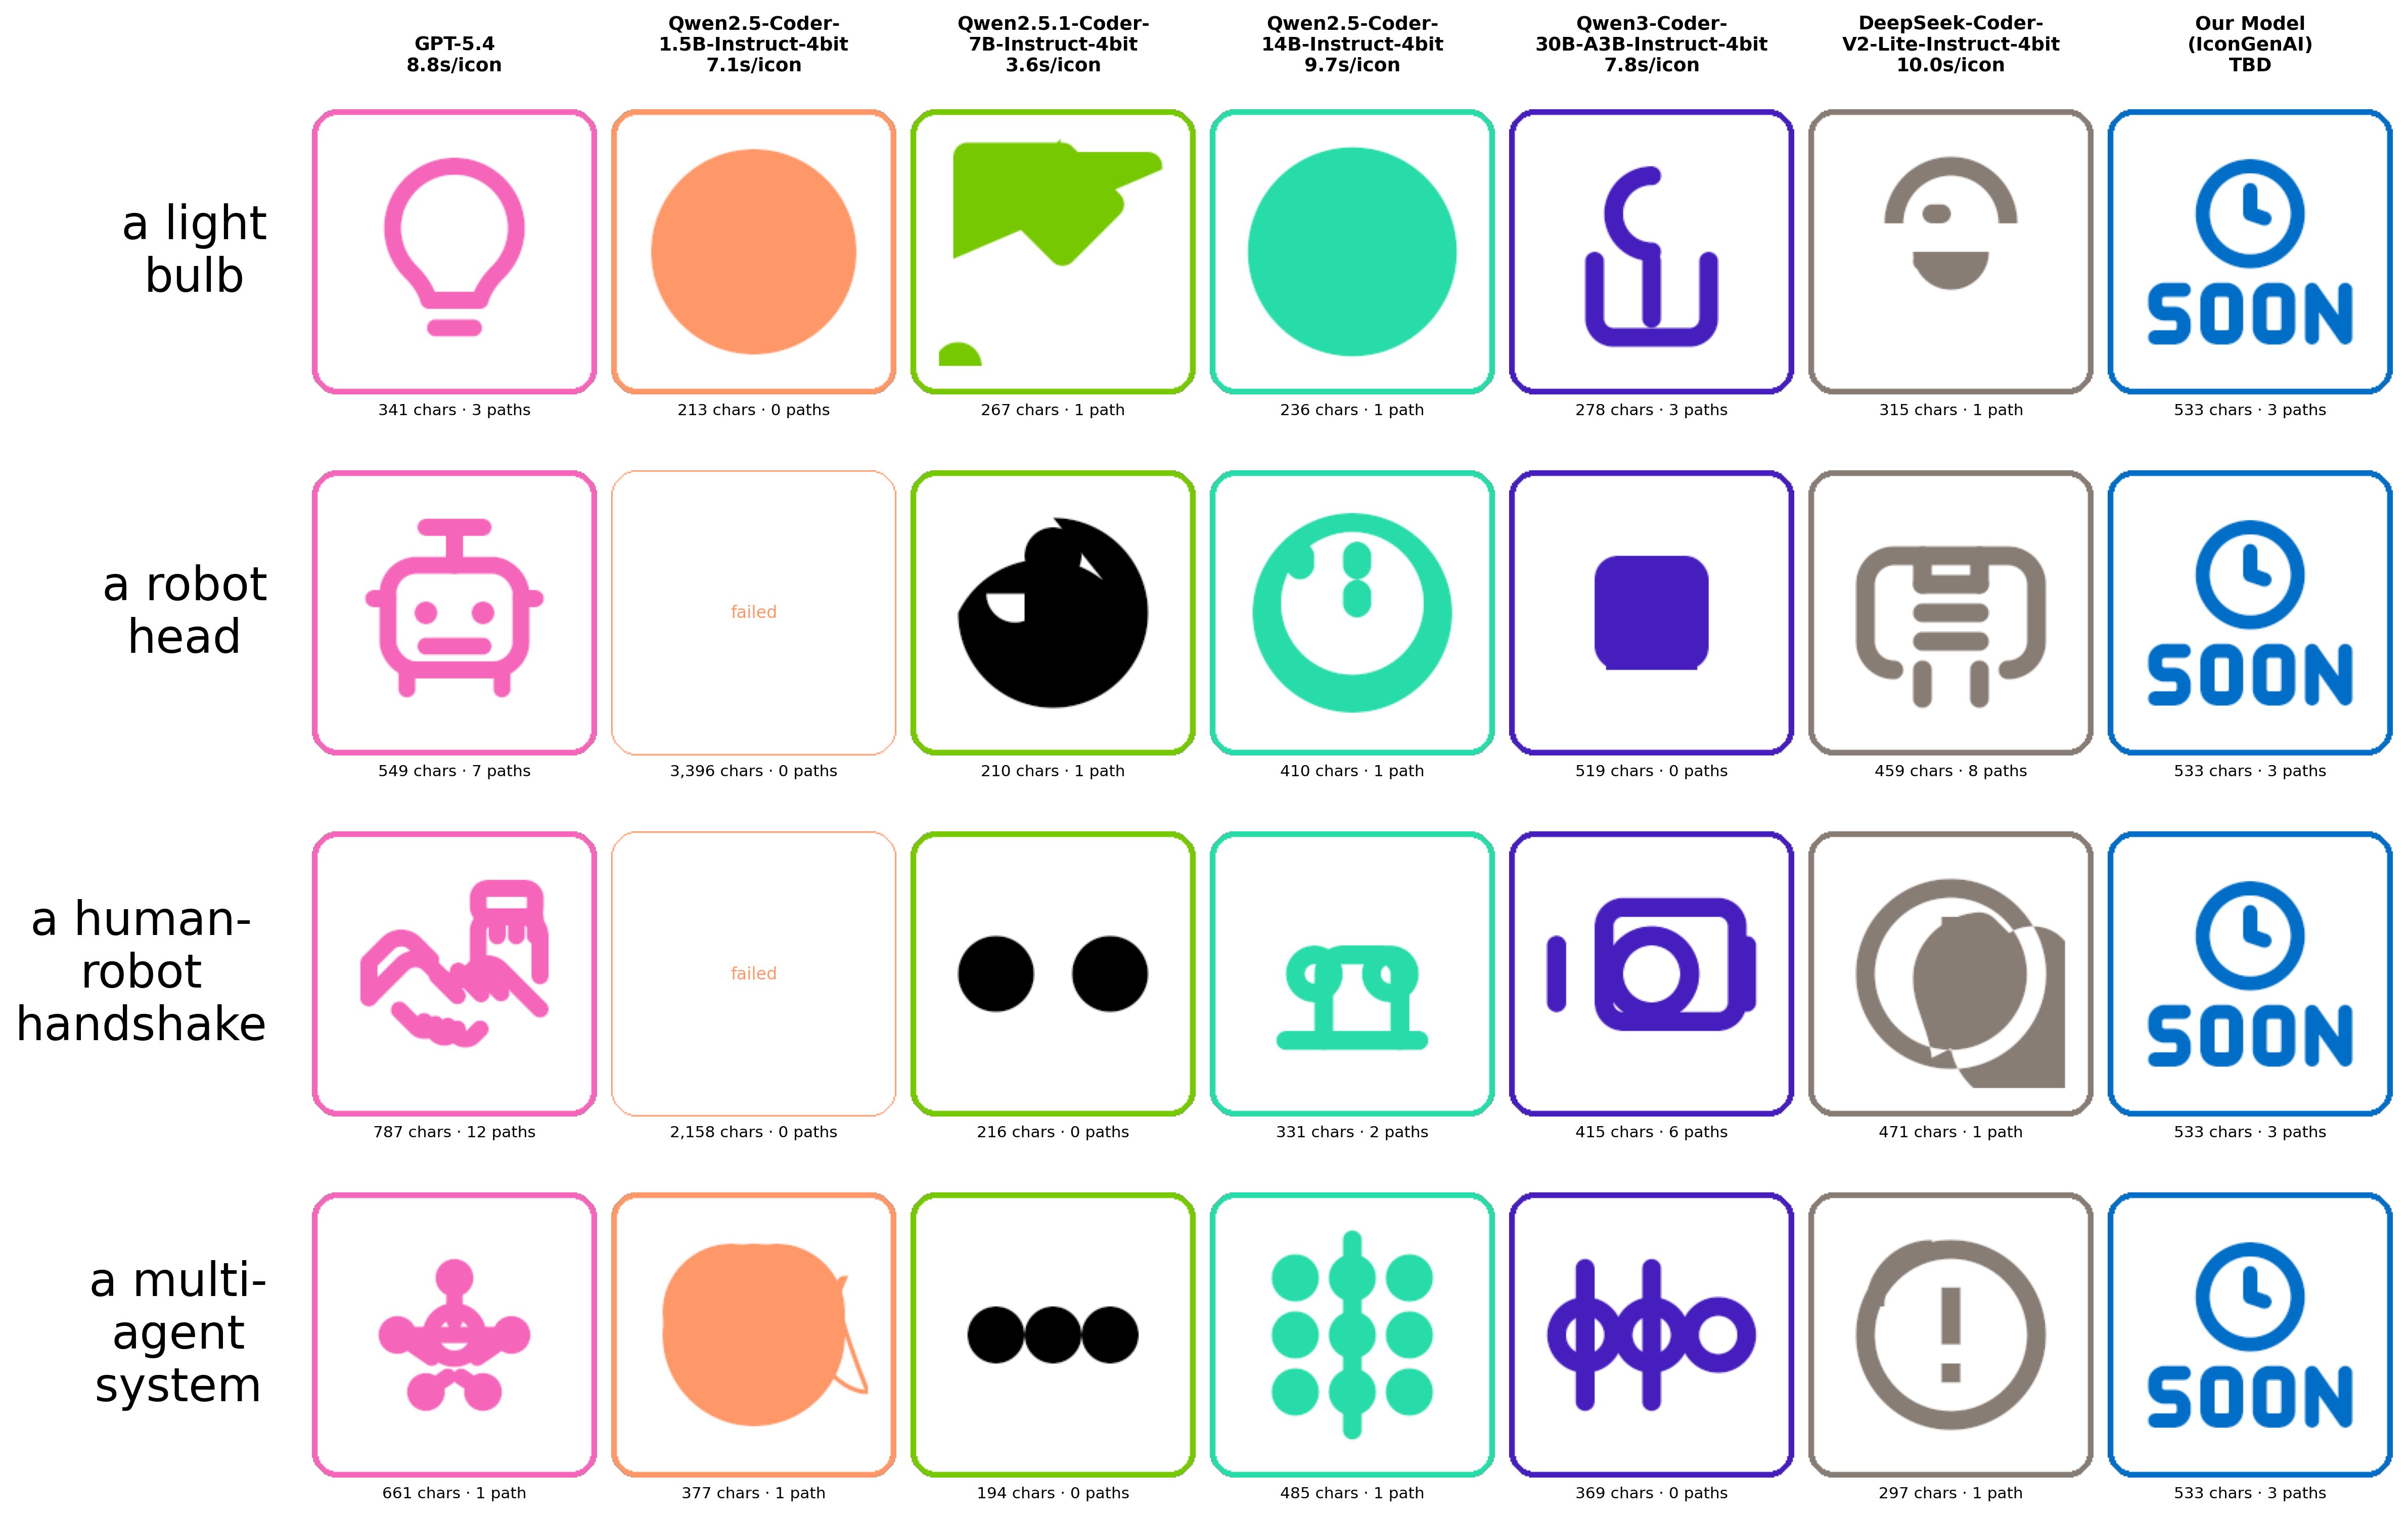
\includegraphics[width=\textwidth]{model_comparison_grid.png}
  \caption{Qualitative comparison of code language models on monochrome SVG icon
           generation. Rows are prompts; columns are models. Each cell shows the
           rendered icon with SVG character count and path count below.
           Our model (\method) column is a placeholder pending fine-tuning.}
  \label{fig:model-comparison}
\end{figure}

% =============================================================================
\begin{abstract}
% ---- Abstract ---------------------------------------------------------------
% Target length: 150–250 words. Write last, once results exist.
% Key elements: problem, gap, approach, dataset, results, significance.

Scalable Vector Graphics (SVG) is the native format for resolution-independent
icons, yet generating high-quality SVG code from natural language descriptions
remains an unsolved problem. Existing text-to-SVG approaches rely on
diffusion-based optimization over rendered pixels, producing outputs that are
slow to generate, difficult to edit, and not constrained to the compact,
semantically clean structure characteristic of professional icons.

We present \textbf{\method}, a domain-specific language model for text-to-SVG
icon generation. Our approach frames icon generation as a structured code
generation task and fine-tunes a pre-trained code language model
(Qwen3.5-9B) using Low-Rank Adaptation (LoRA) on a purpose-built dataset of
natural language and SVG code pairs.

To support this, we introduce the \textbf{\dataset{}} corpus: \num{275912}
SVG icons sourced from the Iconify open-source icon ecosystem, filtered by
license, normalized to a consistent format, and annotated with natural language
descriptions generated by a vision language model (Qwen2.5-VL-7B).

\todo{Fill in: key quantitative results once experiments are complete.
  E.g.: \method{} achieves X\% valid SVG rate, Y CLIP score, outperforming
  StarVector and GPT-4o zero-shot on the icon generation benchmark.}

\method{} generates pixel-perfect, immediately renderable SVG icons in
under one second, enabling practical integration into design tooling and
front-end development workflows. Code, model weights, and the \dataset{}
corpus are released publicly under open-source licenses.

\end{abstract}

% =============================================================================
\section{Introduction}
% ---- Introduction -----------------------------------------------------------
% Target length: ~1 page.
% Structure: (1) problem & motivation, (2) gap in prior work,
%            (3) our approach overview, (4) contributions list.

Icons are the visual vocabulary of modern user interfaces. Every button, menu,
notification, and action is accompanied by a small vector graphic that must
communicate its meaning instantly and scale perfectly from 16 to 512 pixels.
Professional icon libraries --- Heroicons, Material Symbols, Tabler, Lucide ---
contain tens of thousands of carefully crafted SVG files, but they cannot cover
the long tail of application-specific concepts: a domain-specific status
indicator, a company-branded element, or a novel UI affordance.

Generating icons programmatically from natural language would allow designers
and developers to describe what they need --- \textit{"a credit card with three
sparkles in the top right corner"} --- and receive a production-ready SVG file
that renders pixel-perfectly at any resolution and remains fully editable in
vector design tools.

\paragraph{The gap in existing approaches.}
Text-to-image diffusion models \citep{rombach2022ldm, saharia2022imagen} can
produce visually plausible icon-like images, but the output is a raster bitmap,
not a vector graphic. Converting a raster to SVG via auto-tracing produces
imprecise, verbose path data unsuitable for production use. Text-to-SVG methods
based on Score Distillation Sampling \citep{jain2023vectorfusion, xing2024svgdreamer}
optimize Bézier control points to match a target image, yielding semantically
reasonable results for illustrations but generating many redundant paths,
lacking the clean single-path-per-shape structure of handcrafted icons, and
taking tens of seconds per image.

LLM-based SVG generation \citep{rodriguez2025starvector, yang2025omnisvg,
xing2025llm4svg} has recently demonstrated that treating SVG as code leads to
more structured, editable outputs. However, these models are trained on general
SVG corpora covering logos, diagrams, and illustrations --- anime-style artwork,
multi-colour paintings, and raster conversions --- with no focus on icons.

More critically, \emph{no existing model targets monochrome icon generation
specifically}. Professional icon sets --- Heroicons, Material Symbols, Tabler,
Lucide --- use a single semantic colour via the \texttt{currentColor} CSS
property, allowing icons to be instantly recoloured to match any brand or design
system. This monochrome constraint is architecturally distinct from multi-colour
SVG generation: the output is structurally simpler (fewer paths, no gradients,
no colour layers) but semantically demanding --- the silhouette alone must convey
the entire meaning of the icon. This focus on \emph{lightweight, pixel-perfect,
immediately brandable monochrome icons} is what sets our work apart from all
prior text-to-SVG studies.

\paragraph{Our approach.}
We fine-tune Qwen3-Coder-30B \citep{qwen3} --- a state-of-the-art
mixture-of-experts code language model --- on a dataset of \num{275912}
(SVG icon, natural language description) pairs using LoRA \citep{hu2022lora}.
The model is selected from a systematic comparison of Qwen and DeepSeek coder
variants (see Figure~\ref{fig:model-comparison}). The natural language
descriptions are generated automatically by a vision language model
(Qwen2.5-VL-7B \citep{qwen25vl}) applied to rendered PNG images of each icon,
following an established automated annotation pipeline
\citep{rodriguez2025starvector, xing2025llm4svg}.

The resulting model, \textbf{\method}, generates valid, renderable, monochrome
SVG icons in under one second. Unlike diffusion-based approaches, the output
is natively editable, consistently structured, uses \texttt{currentColor} for
immediate brand recolouring, and follows the conventions of professional icon
design and development workflows.

\paragraph{Contributions.}
\begin{enumerate}
    \item \textbf{The \dataset{} Corpus.} A curated dataset of \num{275912}
          SVG icons from the Iconify open-source ecosystem, filtered by license
          (excluding ShareAlike and GPL variants), normalized to a consistent
          SVG format, and annotated with VLM-generated natural language
          descriptions. To our knowledge, this is the first publicly documented
          use of Iconify as a machine learning training corpus.

    \item \textbf{An automated icon annotation pipeline.} A reproducible
          pipeline for rendering SVG icons and generating structured
          short and long natural language descriptions using a vision language
          model, with documented prompt engineering and quality metrics.

    \item \textbf{\method.} A monochrome text-to-SVG model fine-tuned with
          LoRA on Qwen3-Coder-30B, trained specifically for single-colour icon
          generation with curriculum ordering (simple to complex) and
          multi-variant instruction augmentation. The monochrome
          \texttt{currentColor} constraint makes outputs immediately usable
          across any brand or design system.

    \item \textbf{An icon-specific evaluation framework.} Metrics tailored to
          icon generation quality: SVG validity rate, rendering fidelity,
          semantic alignment (CLIP score), and structural economy (path count),
          together with a held-out test set of \num{13795} icons for
          reproducible benchmarking.
\end{enumerate}

Code, model weights, and the \dataset{} corpus are released at:
\url{https://github.com/TODO/icon-genai} under open-source licenses.


% =============================================================================
\section{Related Work}
% ---- Related Work -----------------------------------------------------------
% Target length: ~1.5 pages. Organise into subsections by approach family.
% Cite, describe briefly, and state how this work differs or builds on it.

\subsection{Foundational Vector Graphics Generation}

Early work on learned vector graphics generation treated SVG as a sequence of
drawing commands. \citet{lopes2019svgvae} introduced SVG-VAE, a class-conditioned
variational autoencoder operating on sequential LSTM representations of Bézier
curve commands, trained on 14 million font characters. While limited to simple,
single-glyph shapes, SVG-VAE established the command-sequence paradigm that
most subsequent work adopts.

\citet{carlier2020deepsvg} extended this with DeepSVG, a hierarchical Transformer
that disentangles high-level shape identity from low-level path commands. DeepSVG
introduced a large-scale SVG icon dataset and demonstrated smooth interpolation
and animation of icon sequences, establishing the icon domain as a productive
testbed for vector generation research.

\subsection{Diffusion-Based Text-to-SVG}

The dominant paradigm from 2023--2024 applies Score Distillation Sampling (SDS)
to optimize Bézier path parameters guided by a pretrained text-to-image diffusion
model. VectorFusion \citep{jain2023vectorfusion} demonstrated that a differentiable
rasterizer (DiffVG) can bridge the pixel and vector domains, allowing gradients
from Stable Diffusion to directly update SVG control points. SVGDreamer
\citep{xing2024svgdreamer} improved upon this with Variational Score Distillation
and semantic-driven path initialization, addressing the over-smoothing and
color saturation issues endemic to SDS-based approaches.

These methods produce visually plausible results for illustrations and logos but
are poorly suited to icon generation for three reasons: (1) generation takes
30--120 seconds per image; (2) the optimized paths do not respect icon design
conventions; and (3) the resulting SVG is typically an over-parameterized
approximation rather than a compact, editable structure.

\subsection{LLM-Native SVG Code Generation}

A parallel line of work treats SVG generation as code generation and leverages
the sequence modeling capabilities of large language models. This is the paradigm
our work follows.

IconShop \citep{wu2023iconshop} tokenizes SVG path data into a discrete vocabulary
and trains an autoregressive Transformer on a curated icon corpus. It supports
text-guided generation, interpolation between icons, and semantic combination.
While closely related to our approach, IconShop uses a purpose-built tokenization
scheme and is not built on a pretrained code language model.

StarVector \citep{rodriguez2025starvector} treats image-to-SVG vectorization as
code generation using a Vision-Language Model backbone. Trained on the 2M-sample
SVG-Stack corpus, it handles diverse SVG types including icons, logos, and
technical diagrams. LLM4SVG \citep{xing2025llm4svg} introduces 55 domain-specific
SVG semantic tokens and trains on 250K SVGs with 580K instruction pairs,
demonstrating that structured tokenization improves generation quality.

OmniSVG \citep{yang2025omnisvg} unifies image-conditioned and text-conditioned
generation via a Qwen2.5-VL backbone and the 2M-sample MMSVG-2M dataset. SVGen
\citep{svgen2025} applies Chain-of-Thought reasoning and Group Relative Policy
Optimization (GRPO) reinforcement learning, showing that explicit reasoning
steps significantly improve structural validity.

\paragraph{Distinction from our work.}
All the above LLM-based methods are trained on general SVG corpora and
evaluated on diverse SVG types. We focus exclusively on the icon domain, which
admits a narrower distribution (single-color fills, 1--20 paths, 16--512px
viewBox) and therefore benefits from a specialized training set. We build the
first ML training corpus from the Iconify ecosystem and perform
domain-specific fine-tuning on Qwen3.5-9B, targeting the quality and
structural conventions expected of production icons.

\subsection{Automated SVG Captioning and Datasets}

Several recent works construct large SVG training datasets using automated
annotation pipelines. StarVector \citep{rodriguez2025starvector} renders SVG
files to images and uses a VLM to generate text descriptions, assembling the
SVG-Stack corpus. LLM4SVG \citep{xing2025llm4svg} similarly uses automated
pipelines to produce 580K SVG-text instruction pairs from 250K SVGs. SVGen
\citep{svgen2025} applied this to approximately 500K icons from the Iconfont
repository to produce the SVG-1M dataset.

Our \dataset{} corpus applies the same automated annotation strategy to the
Iconify ecosystem. The key differences are: (1) a rigorous per-set license
filter preserving \num{275912} icons under permissive open-source terms;
(2) use of structured short-and-long caption pairs tuned for instruction
following rather than single descriptions; (3) full documentation of the
normalization pipeline to ensure reproducibility.

\subsection{Evaluation of SVG Generation}

SVGenius \citep{tang2025svgenius} benchmarks 22 LLMs on SVG understanding,
editing, and generation tasks, finding that reasoning-enhanced models outperform
pure scaling and that quality degrades sharply with rising SVG complexity.
VectorGym \citep{vectorgym2025} provides human-annotated benchmarks across four
SVG tasks. Both works confirm the need for domain-specific evaluation metrics
beyond standard image quality scores. Our evaluation framework adapts these
insights to the icon domain.


% =============================================================================
\section{The \dataset{} Corpus}
% ---- Dataset ----------------------------------------------------------------
% Target length: ~1.5 pages.
% Structure: source, collection, license filter, normalization,
%            captioning pipeline, statistics, analysis.

\subsection{Source: The Iconify Ecosystem}

Iconify\footnote{\url{https://iconify.design}} is an open-source meta-library
aggregating over 300,000 icons from 225 icon sets. Unlike individual icon
libraries, Iconify provides a unified JSON format and a public GitHub repository
(\texttt{iconify/icon-sets}) containing all icons as structured data without
requiring web scraping. Each set carries explicit license metadata, making
per-set license filtering straightforward.

\subsection{License Filtering}
\label{sec:license}

Machine learning training use is governed by the license terms of the training
data. We apply a conservative license filter that retains only sets under
permissive open-source licenses and excludes all ShareAlike and copyleft
variants, as detailed in Table~\ref{tab:licenses}.

\begin{table}[h]
\centering
\caption{License filter applied to Iconify collections. ShareAlike and GPL
licenses are excluded due to their potential implications for model weight
distribution.}
\label{tab:licenses}
\begin{tabular}{lrrl}
\toprule
\textbf{License (SPDX)} & \textbf{Sets} & \textbf{Icons} & \textbf{Decision} \\
\midrule
MIT           & 99 & 114,830 & \textcolor{green!60!black}{Include} \\
Apache-2.0    & 30 &  82,644 & \textcolor{green!60!black}{Include} \\
CC-BY-4.0     & 51 &  55,648 & \textcolor{green!60!black}{Include} \\
CC0-1.0       &  8 &   8,051 & \textcolor{green!60!black}{Include} \\
OFL-1.1       & 13 &   6,211 & \textcolor{green!60!black}{Include} \\
CC-BY-3.0     &  1 &   4,123 & \textcolor{green!60!black}{Include} \\
ISC           &  3 &   2,998 & \textcolor{green!60!black}{Include} \\
CC-BY-NC-4.0  &  1 &     479 & \textcolor{green!60!black}{Include (non-commercial)} \\
Unlicense     &  1 &     430 & \textcolor{green!60!black}{Include} \\
MPL-2.0       &  1 &     288 & \textcolor{green!60!black}{Include} \\
BSD-3-Clause  &  1 &     210 & \textcolor{green!60!black}{Include} \\
\midrule
CC-BY-SA-4.0  &  7 &  21,828 & \textcolor{red}{Exclude (ShareAlike)} \\
CC-BY-NC-SA-4.0 & 1 & 1,577 & \textcolor{red}{Exclude (ShareAlike)} \\
CC-BY-SA-3.0  &  2 &      79 & \textcolor{red}{Exclude (ShareAlike)} \\
GPL-*         &  6 &   1,522 & \textcolor{red}{Exclude (Copyleft)} \\
\midrule
\textbf{Total included} & \textbf{209} & \textbf{275,912} & \\
\bottomrule
\end{tabular}
\end{table}

Additionally, 9,045 icons marked as \texttt{hidden} in the Iconify metadata
(deprecated or internal entries) are excluded, and alias entries (icons defined
as references to parent icons) are skipped to avoid duplicate training samples.

This study is conducted for non-commercial research purposes. Beyond license
terms, we note that (1) the EU DSM Directive (Article 4) explicitly permits
text and data mining of lawfully accessed content for research use; (2) the
trained model weights are a derivative work that does not reproduce training
icons verbatim. Each record in the released dataset retains the original
Iconify metadata fields \texttt{collection\_name}, \texttt{license\_spdx},
\texttt{author}, and \texttt{license\_url}, enabling downstream users to
comply with the attribution requirements of CC-BY and similar licenses.

\subsection{SVG Normalization}

Raw Iconify data consists of SVG \texttt{body} fragments — the inner content
of the \texttt{<svg>} element without the root tag or namespace declaration.
We assemble each icon into a complete, valid SVG document:

\begin{lstlisting}[style=svgstyle, caption={Assembled SVG document format}]
<svg xmlns="http://www.w3.org/2000/svg"
     viewBox="0 0 {W} {H}" width="{W}" height="{H}">
  {body}
</svg>
\end{lstlisting}

Two color conventions appear in the corpus. \emph{Monochrome} icons (the
majority) use \texttt{currentColor} as the fill and stroke value — the
standard convention in icon design that allows the icon to inherit its
context's text color. \emph{Multicolor} icons contain explicit color values
(hex codes, named colors, or \texttt{rgb()} expressions) hardcoded in the
path elements, e.g.\ \texttt{fill="\#4285F4"}. Each record carries an \texttt{is\_multicolor} boolean flag computed by
scanning the SVG body for explicit color values (hex codes, \texttt{rgb()},
or the named colors \texttt{white}/\texttt{black}) outside any
\texttt{currentColor} reference. This flag is used during curriculum
ordering (Section~\ref{sec:curriculum}) to expose the model to simple
monochrome icons before the more complex multicolor ones.

\subsection{Automated Caption Generation}
\label{sec:captioning}

Natural language descriptions are generated using Qwen2.5-VL-7B-Instruct
\citep{qwen25vl}, a vision language model running on Apple Silicon via the
MLX framework \citep{mlx2023}. Each icon is rendered to a 256$\times$256 PNG
using CairoSVG and passed to the VLM with a structured prompting template.

We generate two caption variants per icon:

\begin{itemize}
    \item \textbf{Short caption (5--12 words):} a natural search query expressing
          the concept and visual style, e.g., \textit{"outlined credit card with
          sparkles"} or \textit{"filled shopping cart with checkmark badge"}.
          This serves as the primary training prompt.
    \item \textbf{Long caption (20--35 words):} a detailed description including
          visual style (outline/filled/flat/solid/line), all visible elements,
          any decorations or modifiers, and likely UI context.
\end{itemize}

The icon name and collection name from Iconify metadata are provided as context
in the prompt, helping the model identify the semantic intent of ambiguous icons.
Caption generation runs checkpointed at the icon level, enabling resumable
processing across multiple sessions.

\todo{Report: total captioning time, model throughput, fraction of icons
requiring fallback to icon name (parse failure rate).}

\subsection{Dataset Statistics}

\todo{Add figures once captioning is complete:
(1) distribution of path\_count (histogram);
(2) proportion monochrome vs. multicolor by collection;
(3) caption length distribution (short and long);
(4) most frequent concepts in short captions (word cloud or bar chart);
(5) sample grid of icons across collections.}

Table~\ref{tab:dataset_stats} summarises the key characteristics of the
\dataset{} corpus.

\begin{table}[h]
\centering
\caption{\dataset{} corpus statistics.}
\label{tab:dataset_stats}
\begin{tabular}{lr}
\toprule
\textbf{Attribute} & \textbf{Value} \\
\midrule
Total icons            & 275,912 \\
Icon sets              & 209 \\
Monochrome icons       & \todo{X\%} \\
Multicolor icons       & \todo{X\%} \\
Median path count      & \todo{X} \\
Mean path count        & \todo{X} \\
Mean short caption length (words) & \todo{X} \\
Mean long caption length (words)  & \todo{X} \\
Training split         & 248,120 (90\%) \\
Validation split       &  13,896  (5\%) \\
Test split             &  13,896  (5\%) \\
\bottomrule
\end{tabular}
\end{table}


% =============================================================================
\section{Method}
% ---- Method -----------------------------------------------------------------
% Target length: ~1 page.
% Structure: SVG representation, base model, training formulation, LoRA, curriculum.

\subsection{SVG as Code}

SVG is an XML-based language for describing two-dimensional vector graphics.
An icon SVG typically consists of a root \texttt{<svg>} element with a
\texttt{viewBox} attribute defining the coordinate space, followed by one or
more geometric primitives: \texttt{<path>} elements with \texttt{d} attributes
encoding sequences of drawing commands (MoveTo, LineTo, CubicBézier,
EllipticalArc, ClosePath), and optionally \texttt{<circle>}, \texttt{<rect>},
\texttt{<polygon>}, or \texttt{<g>} grouping elements.

This structure is naturally representable as a text sequence, and modern code
language models pre-trained on source code corpora have already seen XML and
SVG-like content in their training data. We leverage this prior knowledge by
treating icon generation as instruction-following code generation: given a
natural language description as the user instruction, produce a complete,
valid SVG document as the assistant response.

\subsection{Base Model}

We use Qwen3.5-9B \citep{qwen3} as the base model. Qwen3.5 represents the
current generation of Qwen language models \citep{qwen25}, featuring a 128K
token context window (important for complex SVGs), strong performance on code
generation benchmarks, and native instruction-following capabilities through
the ChatML prompt format. The 9B parameter scale balances generation quality
with the memory and compute constraints of local Apple Silicon hardware.

\subsection{Instruction-Tuning Formulation}

Each training example is formatted as a three-turn conversation in the
ChatML format used by Qwen3.5:

\begin{lstlisting}[style=svgstyle, caption={Training record format (ChatML)}]
{"messages": [
  {"role": "system",
   "content": "You are an SVG icon generator. Given a description,
               output clean, valid SVG code for a single icon. Use
               currentColor for fill and stroke. Output only the
               SVG element, no explanation."},
  {"role": "user",
   "content": "Generate an SVG icon: outlined credit card with sparkles"},
  {"role": "assistant",
   "content": "<svg xmlns=... viewBox=...><path .../></svg>"}
]}
\end{lstlisting}

\subsection{Data Augmentation}

For each icon we generate up to three training variants with different
user-side prompts pointing to the same SVG target:
(1) the short VLM caption (\textit{"outlined credit card with sparkles"}),
(2) the long VLM caption (full description with style and context), and
(3) the raw icon name from the Iconify metadata (\textit{"credit-card"}).
This teaches the model to handle prompts of varying specificity and phrasing,
reflecting the diversity of real-world user queries.

\subsection{Curriculum Learning}
\label{sec:curriculum}

Following \citet{svgen2025}, training examples are ordered from simple to
complex using a two-level sort key: (1) monochrome icons before multicolor,
(2) ascending path count within each group. This curriculum strategy exposes
the model to the dominant icon patterns first, grounding its SVG priors before
introducing the long-tail of complex multicolor icons.

\subsection{LoRA Fine-tuning}
\label{sec:lora}

We apply Low-Rank Adaptation \citep{hu2022lora} to fine-tune Qwen3.5-9B,
keeping the pre-trained weights frozen and adding trainable low-rank matrices
$A \in \mathbb{R}^{d \times r}$ and $B \in \mathbb{R}^{r \times d}$ at each
attention and MLP projection layer. The effective weight update is:

\[
W' = W + \alpha \cdot A B
\]

where $r$ is the rank (we use $r = 64$) and $\alpha$ is a scaling factor.
With 4-bit quantization of the frozen base weights (QLoRA), total GPU memory
is under 16~GB, enabling training on Apple M4 hardware via the MLX framework
\citep{mlx2023}.

\paragraph{Training configuration.}
\todo{Fill in after training:
batch size, learning rate, number of iterations, hardware, training time per epoch.}
Table~\ref{tab:training_config} summarises the training hyperparameters.

\begin{table}[h]
\centering
\caption{Training configuration for \method{}.}
\label{tab:training_config}
\begin{tabular}{ll}
\toprule
\textbf{Hyperparameter} & \textbf{Value} \\
\midrule
Base model      & Qwen3.5-9B-Instruct \\
Quantization    & 4-bit (QLoRA) \\
LoRA rank $r$   & 64 \\
LoRA $\alpha$   & 128 \\
LoRA target layers & attention + MLP projections \\
Training epochs & 2--3 \\
Batch size      & \todo{X} \\
Learning rate   & \todo{X} \\
Training records & \todo{X} (with augmentation) \\
Hardware        & Apple M4 / \todo{cloud GPU} \\
Training time   & \todo{X hours} \\
\bottomrule
\end{tabular}
\end{table}


% =============================================================================
\section{Experiments}
% ---- Experiments ------------------------------------------------------------
% This section is largely a TODO until training and evaluation are complete.
% Write the setup and metrics now; fill in results later.

\todo{This section is a template. Fill in all tables and results after
training and evaluation are complete.}

\subsection{Evaluation Metrics}

We evaluate on the held-out test split of 13,896 icons. For each test icon,
the model receives the short VLM caption as the prompt and generates SVG code.
We measure the following:

\begin{itemize}
    \item \textbf{SVG Validity Rate (VR):} fraction of generated outputs that
          parse as well-formed XML with a valid root \texttt{<svg>} element.
          A model that generates syntactically broken SVG is unusable.

    \item \textbf{Rendering Success Rate (RSR):} fraction of valid SVGs that
          render without errors using CairoSVG. Catches semantic issues such
          as malformed \texttt{d} attributes that parse as XML but fail to render.

    \item \textbf{CLIP Score:} cosine similarity between the CLIP \citep{radford2021clip}
          embedding of the rendered icon PNG and the CLIP embedding of the
          text prompt, measuring semantic alignment. We use
          ViT-B/32 \citep{radford2021clip} as the backbone.

    \item \textbf{Mean Path Count (MPC):} average number of \texttt{<path>}
          elements in generated icons. Lower is preferable; professional icons
          typically use 1--5 paths. This measures structural economy.

    \item \textbf{FID (Fréchet Inception Distance):} distributional similarity
          between rendered generated icons and rendered ground-truth icons,
          computed over the test split. Lower is better.
\end{itemize}

\subsection{Baselines}

We compare against two categories of baseline.
\textit{Zero-shot LLM baselines} are general-purpose language models prompted
with the same system and user messages as \method{}, but without any
SVG-specific fine-tuning; the ``(zero-shot)'' label distinguishes these from
models that were explicitly trained for SVG generation.
\textit{Supervised SVG baselines} are models trained end-to-end on SVG
corpora and represent the current open-weight state of the art.

\begin{itemize}
    \item \textbf{Qwen3.5-9B (zero-shot):} the base model without fine-tuning,
          prompted identically to \method{}. Isolates the contribution of
          domain-specific fine-tuning.

    \item \textbf{GPT-5.4 (zero-shot):}
          OpenAI's GPT-5.4 prompted via the API with the same prompts.
          Serves as a strong commercial LLM reference point.
          Parameter count is not publicly disclosed.

    \item \textbf{StarVector-8B} \citep{rodriguez2025starvector}: an
          8B-parameter open-weight model that frames SVG generation as
          code generation from a vision-language backbone; state of the art
          on general SVG vectorization at the time of writing.

    \item \textbf{OmniSVG-8B} \citep{yang2025omnisvg}: 8B-parameter model
          trained on MMSVG-2M including a dedicated icon subset, making it
          the most directly comparable supervised baseline.
\end{itemize}

\subsection{Quantitative Results}

\todo{Fill in Table~\ref{tab:main_results} once evaluation is complete.}

\begin{table}[h]
\centering
\caption{Main results on the \dataset{} test split. Best results in \textbf{bold}.}
\label{tab:main_results}
\begin{tabular}{lrccccc}
\toprule
\textbf{Model} & \textbf{Params} & \textbf{VR (\%)} & \textbf{RSR (\%)} & \textbf{CLIP $\uparrow$} & \textbf{MPC $\downarrow$} & \textbf{FID $\downarrow$} \\
\midrule
\multicolumn{7}{l}{\textit{Commercial zero-shot}} \\
\quad GPT-5.4                        & n/a           & \todo{} & \todo{} & \todo{} & \todo{} & \todo{} \\
\multicolumn{7}{l}{\textit{Open-weight zero-shot}} \\
\quad Qwen3.5-\todo{1.7B or 9B}      & \todo{1.7B or 9B} & \todo{} & \todo{} & \todo{} & \todo{} & \todo{} \\
\multicolumn{7}{l}{\textit{SVG-specific (supervised)}} \\
\quad StarVector-8B                  & 8B            & \todo{} & \todo{} & \todo{} & \todo{} & \todo{} \\
\quad OmniSVG-8B                     & 8B            & \todo{} & \todo{} & \todo{} & \todo{} & \todo{} \\
\midrule
\textbf{\method{} (ours)}            & \todo{1.7B or 9B} & \todo{} & \todo{} & \todo{} & \todo{} & \todo{} \\
\bottomrule
\end{tabular}
\end{table}

\subsection{Ablation Studies}

\todo{Run and fill in Table~\ref{tab:ablation} once training is complete.}

\begin{table}[h]
\centering
\caption{Ablation study on key design decisions.}
\label{tab:ablation}
\begin{tabular}{lcccc}
\toprule
\textbf{Variant} & \textbf{VR (\%)} & \textbf{RSR (\%)} & \textbf{CLIP $\uparrow$} & \textbf{FID $\downarrow$} \\
\midrule
\method{} (full)           & \todo{} & \todo{} & \todo{} & \todo{} \\
\quad w/o curriculum       & \todo{} & \todo{} & \todo{} & \todo{} \\
\quad w/o augmentation     & \todo{} & \todo{} & \todo{} & \todo{} \\
\quad short captions only  & \todo{} & \todo{} & \todo{} & \todo{} \\
\quad 1 epoch (vs.\ 3)     & \todo{} & \todo{} & \todo{} & \todo{} \\
\bottomrule
\end{tabular}
\end{table}


% =============================================================================
\section{Analysis}
% ---- Analysis ---------------------------------------------------------------
% Write qualitative analysis after training. Placeholders for now.

\subsection{Qualitative Examples}

\todo{Insert a figure grid: 3--4 rows of (prompt, generated SVG, ground-truth icon)
showing representative successes across icon styles.
Row 1: simple monochrome outline icons (e.g., arrows, UI actions)
Row 2: multicolor icons or icons with badges/decorators
Row 3: abstract/metaphorical icons (e.g., "speed", "security")
Row 4: multi-element compositions}

\begin{figure}[h]
    \centering
    \todo{Insert figure: qualitative\_examples.pdf}
    \caption{Representative \method{} outputs alongside their prompts
    and the closest ground-truth icons from the test split.}
    \label{fig:qualitative}
\end{figure}

\subsection{Failure Modes}

\todo{Analyse and describe after evaluation. Expected failure cases based on
prior work and dataset properties:}

\begin{itemize}
    \item \textbf{Rare or abstract concepts} — icons for uncommon concepts
          (e.g., domain-specific technical symbols) that appear infrequently
          in training may produce generic or semantically misaligned outputs.

    \item \textbf{Complex multi-element compositions} — icons described as
          having more than 3--4 distinct visual elements tend to have lower
          rendering fidelity, consistent with the SVGenius finding that quality
          degrades with rising SVG complexity.

    \item \textbf{Invalid path data} — occasionally the model generates
          syntactically plausible but geometrically malformed \texttt{d}
          attributes (e.g., missing coordinate pairs after a command letter).
          This manifests as rendering errors. \todo{Quantify rate.}

    \item \textbf{ViewBox mismatch} — some generated icons place content
          outside the declared viewBox, resulting in clipped rendering.
\end{itemize}

\subsection{Caption Quality Ablation}

\todo{Compare: (1) VLM-generated captions vs. (2) raw icon names as prompts
for fine-tuning. This isolates the contribution of the captioning pipeline.}

\subsection{Comparison with General SVG Models}

\todo{Discuss qualitative differences between \method{} and StarVector/OmniSVG
on icon-specific prompts. Hypothesis: general models produce more complex,
less icon-like SVG structure; \method{} produces compact, \texttt{currentColor}
convention-following icons consistent with professional icon libraries.}


% =============================================================================
\section{Conclusion}
% ---- Conclusion -------------------------------------------------------------
% Write last. Short (~0.5 page): restate contributions, key finding, future work.

\todo{Write after experiments are complete. Draft outline:}

We presented \method{}, a domain-specific language model for text-to-SVG icon
generation. We introduced the \dataset{} corpus --- \num{275912} license-filtered,
normalized SVG icons from the Iconify ecosystem, annotated with VLM-generated
natural language descriptions --- and demonstrated that LoRA fine-tuning of
Qwen3.5-9B on this corpus yields a model that generates valid, renderable,
semantically aligned SVG icons from natural language prompts.

\todo{Insert key numerical finding.}

\paragraph{Limitations.}
The \dataset{} corpus reflects the distribution of the Iconify ecosystem:
predominantly single-color, geometric icons in flat or outline styles. The
model may generalize poorly to photorealistic SVGs, complex illustrations,
or icon styles not represented in Iconify. Caption quality depends on the
vision model and prompt template; a small fraction of icons receive semantically
inaccurate descriptions that may reduce training signal quality.

\paragraph{Future work.}
We identify three promising directions. First, incorporating reasoning-enhanced
training \citep{svgen2025, reason_svg2025} via GRPO reinforcement learning may
further improve structural validity without increasing dataset size. Second,
interactive editing --- given an existing icon and a textual modification
instruction, produce an updated SVG --- is a natural extension enabled by the
instruction-following formulation. Third, evaluating the model in a
user study with designers and front-end developers would provide ecological
validity beyond the automated metrics used here.


% =============================================================================
\printbibliography

\end{document}
